\section{Experiments}
\label{sec:experiments}


We performed an experimental analysis of our proposed algorithm on real-life and synthetic datasets considering realistic scenarios. We first examine the effect of different parameters on the running time. 
We show that our solution scales, performs well on realistic scenarios and that the optimization presented in Section~\ref{sec:optimizations} are effective. We then compare our solution to~\cite{MLJ22,ERICA} that studies a similar problem for queries without ranking. We demonstrate the differences between solutions and compare their outputs and performance through a use case.
 



\begin{table*}[t!]
    \centering
    \footnotesize
    \caption{Queries and constraints}
    \scalebox{0.72}{
        \begin{tabular}{lclcl}
        \hline
        \textbf{Dataset} & \textbf{Query} & \multicolumn{1}{c}{\textbf{Predicates}} & \textbf{Order by (DESC)} & \multicolumn{1}{c}{\textbf{Constraints}}\\ \hline\hline
        Astronauts & $Q_A$ & 
        \begin{tabular}{l@{}}\texttt{"Graduate Major" = 'Physics'}\\ \texttt{AND "Space Walks" <= 3}\\ \texttt{AND "Space Walks" >= 1} \end{tabular}  
        &{\tt "Space Flight (hrs)"}&\begin{tabular}{@{}ll@{}}
            (1) $\lb{Gender='F'}{k} = \frac{k}{2}$ & (4) $\lb{Status='Management'}{k} = \frac{k}{5}$ \\ (2) $\lb{Gender='M'}{k} = \frac{k}{2}$ & (5) $\lb{Status='Retired'}{k} = \frac{k}{5}$ \\ (3) $\lb{Status='Active'}{k} = \frac{k}{5}$ &
        \end{tabular}\\
        \hline
        Law Students & $Q_L$ & \begin{tabular}{l@{}}\texttt{Region = 'GL'}\\\texttt{AND GPA <= 4.0}\\\texttt{AND GPA >= 3.5}\end{tabular}& {\tt LSAT}&\begin{tabular}{@{}ll@{}}
            (1) $\lb{Sex='F'}{k} = \frac{k}{2}$ & (4) $\lb{Race='White'}{k} = \frac{k}{5}$ \\ (2) $\lb{Sex='M'}{k} = \frac{k}{2}$ & (5) $\lb{Race='Asian'}{k} = \frac{k}{5}$ \\ (3) $\lb{Race='Black'}{k} = \frac{k}{5}$ &
        \end{tabular}\\
       \hline
        MEPS & $Q_M$ & \begin{tabular}{l@{}}\texttt{Age > 22}\\\texttt{AND "Family Size" >= 4}\end{tabular}& {\tt Utilization}&\begin{tabular}{@{}ll@{}}
            (1) $\lb{Sex='F'}{k} = \frac{k}{2}$ & (4) $\lb{Race='Black'}{k} = \frac{k}{5}$ \\ (2) $\lb{Sex='M'}{k} = \frac{k}{2}$ & (5) $\lb{Race='White'}{k} = \frac{k}{5}$ \\ (3) $\lb{Race='Asian'}{k} = \frac{k}{5}$ &
        \end{tabular}\\ \hline
        TPC-H & $Q_5$ & \begin{tabular}{l@{}}\texttt{Region = 'ASIA'}\end{tabular} & {\tt Revenue}& \begin{tabular}{@{}ll@{}}
            (1) $\lb{OrderPrio='5-LOW'}{k} = \frac{k}{2}$ & (4) $\lb{MktSeg='BUILDING'}{k} = \frac{k}{5}$ \\ (2) $\lb{OrderPrio='3-MEDIUM'}{k} = \frac{k}{5}$ & (5) $\lb{MktSeg='MACHINERY'}{k} = \frac{k}{5}$ \\ (3) $\lb{MktSeg='AUTOMOBILE'}{k} = \frac{k}{5}$ &
        \end{tabular}\\ \hline
        \end{tabular}
    }
    \label{tab:queriesAndConstraints}
\end{table*}


\subsection{Evaluation Benchmark}\label{sec:benchmark}
To the best of our knowledge, we are the first to consider this problem, and there is no benchmark consisting of datasets, including ranking queries and sets of cardinality constraints. To this end, we have developed a dedicated benchmark that involves real-life datasets used in the context of ranking as follows. 
\begin{itemize}[leftmargin=1em,labelwidth=*,align=left]
    \item {\bf Astronauts\footnote{\url{https://www.kaggle.com/datasets/nasa/astronaut-yearbook}}}: A dataset of 19 attributes containing 357 NASA astronauts and information about their careers. Astronauts are ranked in descending order by their number of space flight hours, as was done in \cite{SYJ18}.
    \item {\bf Law Students \cite{LawDataOriginal,LawData}}: A dataset of 8 attributes containing 21,790 law students and various evaluations such as grade point average, LSAT examination scores, and first year grade average. Students are ranked by their LSAT scores, as in \cite{ZHW20}.
    \item {\bf MEPS\footnote{\url{https://meps.ahrq.gov/data\_stats/download\_data/pufs/h192/h192doc.shtml}}}: A dataset of 1,941 attributes containing 34,655 individuals and information related to their usage of healthcare. Patients are ranked in descending order by a combination of utilization metrics (office-based visits + ER visits + in-patient nights + home health visits), as was done in~\cite{YGS19}. 
\end{itemize}

To evaluate scalability, we use Synthetic Data Vault (SDV) \cite{SDV} to learn the distributions of our real-life datasets and subsequently synthesize scaled-up versions.
We also use the {\bf TPC-H Benchmark}%
, which includes complex queries involving multiple tables. We generate a TPC-H dataset of scale factor $1$, which is approximately $1$ GB of data. We use Query 5 (Q5) from the TPC-H specification and remove the predicates filtering on date types. 















\paragraph*{\textbf{Queries and constraints}} %
\Cref{tab:queriesAndConstraints} summarizes the queries and constraints used.
 We generated queries and constraints for each dataset, showcasing real-life scenarios. Each row in the table represents a query. %
 For example, the first line represents the following query 
 $Q_A$ over the Astronauts dataset. 
 \begin{center}
     \footnotesize
     \begin{tabular}{l}
        \verb"SELECT * FROM Astronauts" \\
        \verb|WHERE "Space Walks" <= 3 AND "Space Walks" >= 1| \\
        \verb|AND "Graduate Major" = 'Physics'|\\
        \verb|ORDER BY "Space Flight (hrs)" DESC|\\
     \end{tabular}
     \end{center}
     This query may be used in the selection process of astronauts for a mission. The mission requires specific training (number of space walks) and background (graduate major), and the candidates are ordered by their experience (space flight hours).  
     Similarly, the query $Q_L$ for the Law Students dataset may be used to rank outstanding students (based on their GPA) from a particular region based on their SAT scores for a scholarship. Finally, $Q_M$ is defined for the MEPS dataset.  Such a query may be used to invite the best-fitting patients (based on their utilization) with specific criteria, for a study.
     
     
     
     We defined result diversity constraints for each dataset (listed in Table~\ref{tab:queriesAndConstraints}). For instance, in the Astronauts dataset, the result should include women and candidates of varying ranks in the organizational hierarchy. The constraints' bounds are parameterized with a value $k$, and we set them to values that produce a valid refinement in most cases. Specifically, out of 132 performed experiments, we were not able to find a solution in only 2. 
     

 


\paragraph*{\textbf{Parameters setting}} When using ranked-retrieval in decision-making contexts (e.g., when deciding how many people to invite for in-person interviews), one expects the number of items a user will consider ($k$) to be relatively low. In general, rankings are subject to position bias --- a geometric drop in visibility of items in lower ranks --- and so are best-suited for cases where the user interacts with a small number of top-ranked items~\cite{DBLP:journals/cacm/Baeza-Yates18}.
Thus, unless otherwise specified, we use $k=10$ as a default value. Furthermore, we let the default maximum deviation $\varepsilon$ be $0.5$, aiming to strike a balance between being sufficiently close to the constraints but realistically possible in the datasets. In practice, this parameter may be chosen by specifying a worst-case scenario that is still acceptable, and then use the deviation of this scenario as calculated by \Cref{def:mospe} to set $\varepsilon$. We also set the constraints set to include a single constraint (constraint (1) from Table~\ref{tab:queriesAndConstraints} for each dataset). We used the three distance measures mentioned in \Cref{sec:distance}: the queries predicates distance measure $DIS_{pred}$ (abbr. QD in the figures), the Jaccard distance over the output, $DIS_{Jaccard}$ (JAC in the figures), and Kendall's $\tau$, $DIS_{Kendall}$, for top-$k$ lists defined in~\cite{FKS03} (KEN in the figures). 





\paragraph*{\textbf{Compared algorithms}}
To our knowledge, our problem is novel and has no competing algorithms other than the na\"{i}ve exhaustive search. Therefore, we compare our baseline MILP-based algorithm (MILP), our optimized MILP-based algorithm (MILP+opt), which includes the optimization described in Section~\ref{sec:optimizations}, an exhaustive search over the space of refinements (Na\"{i}ve), and a version the exhaustive search that uses our provenance annotations to evaluate the refinements (Na\"{i}ve+prov). 
We report the total running time and show the setup time (constructing the MILP for MILP-based solutions, and generating the provenance for Na\"{i}ve+prov). The MILP solver time is the gap between total and setup.
The reported times are an average of $5$ executions.

 

\paragraph*{\textbf{Platform \& implementation details}}
Our experiments were performed on macOS 13.4 with an Apple M2 processor and 16 GB of memory. Our algorithm was implemented with IBM's CPLEX 22.1.1.0\footnote{\url{https://www.ibm.com/products/ilog-cplex-optimization-studio/cplex-optimizer}} to solve the mixed-integer linear program and DuckDB 0.8.0 \cite{DuckDB} for query evaluation. The algorithm to construct the problem and the na\"{i}ve method were written and evaluated with Python 3.9.6 and PuLP 2.7.0 (the library used for modeling the MILP problem). $DIS_{pred}$ is linearized by computing the Jaccard distance for categorical predicates through the Charnes-Cooper transformation~\cite{CC62}. In addition, for numerical predicates, additional variables are generated that represent the absolute difference between the refined and original constants. As it does not consider the output, we skip generating $s_t$ and $l_{t, k}$ variables for tuples that do not belong to any group $G$ in $\constraints$. $DIS_{Jaccard}$ is evaluated over the output, thus we leverage the fact that there are at least $k^*$ tuples in the output and aim at maximizing the number of original tuples output, thereby maximizing the Jaccard distance.
For $DIS_{Kendall}$, only Cases 2 (a tuple leaves the top-$k$) and 3 (a tuple enters the top-$k$) as defined in \cite{FKS03} may occur in our model. We create a variable for each case for each tuple, which is then equal to the sum of the case if the tuple is selected and zero otherwise. For more details, see~\cite{Extended, impl}.





\subsection{Results}\label{sec:results}

\begin{figure}[t]
    \begin{subfigure}{.35\textwidth}
      \centering
      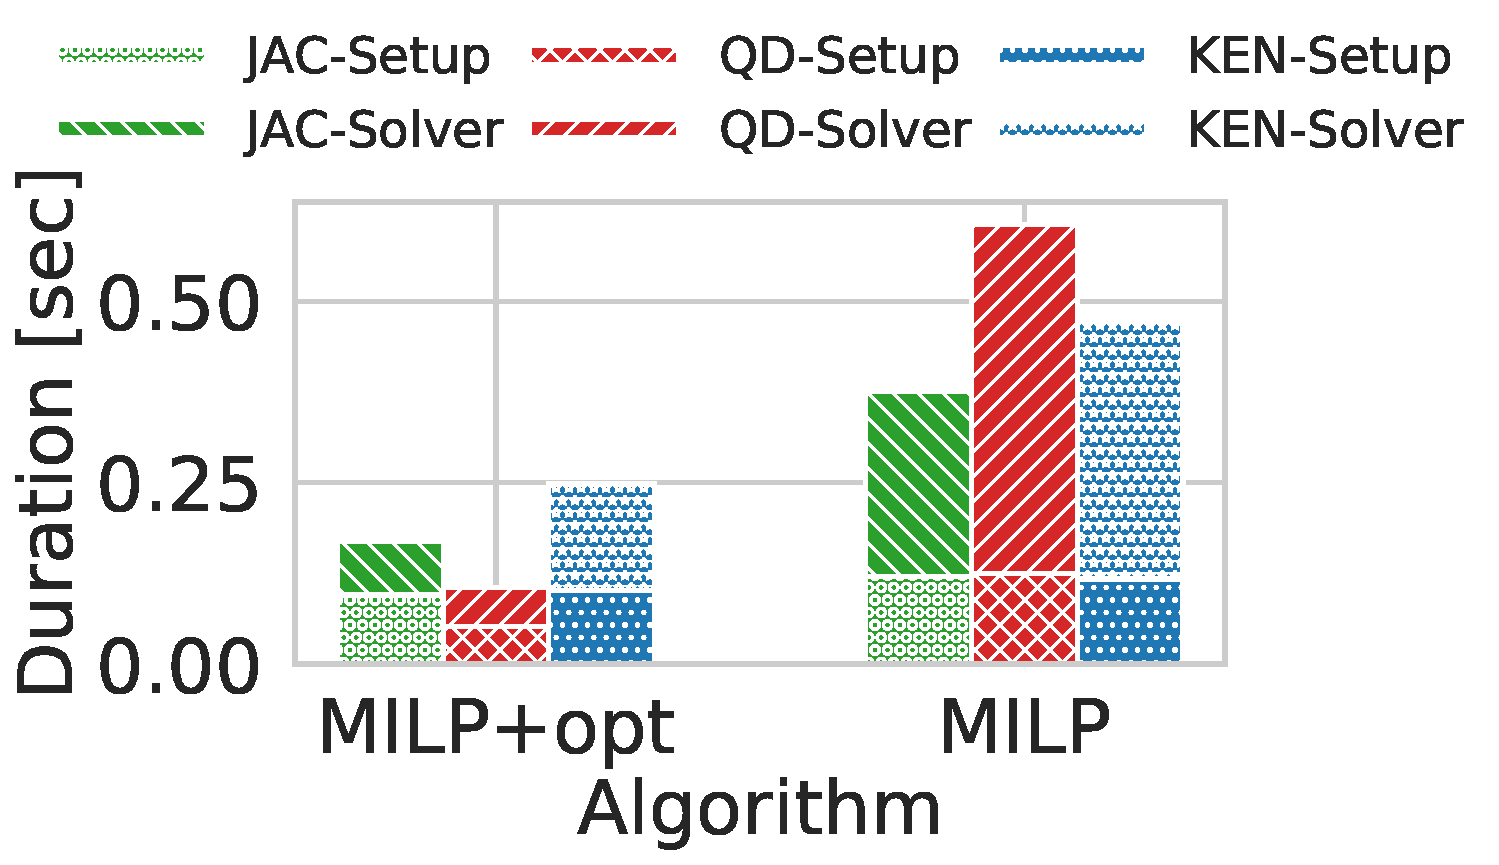
\includegraphics[width=.87\linewidth]{figures/astr_method.pdf}
      \hspace{-0.6cm}
      \caption{Astronauts}
      \label{fig:r1}
    \end{subfigure}%
    \begin{subfigure}{.35\textwidth}
      \centering
      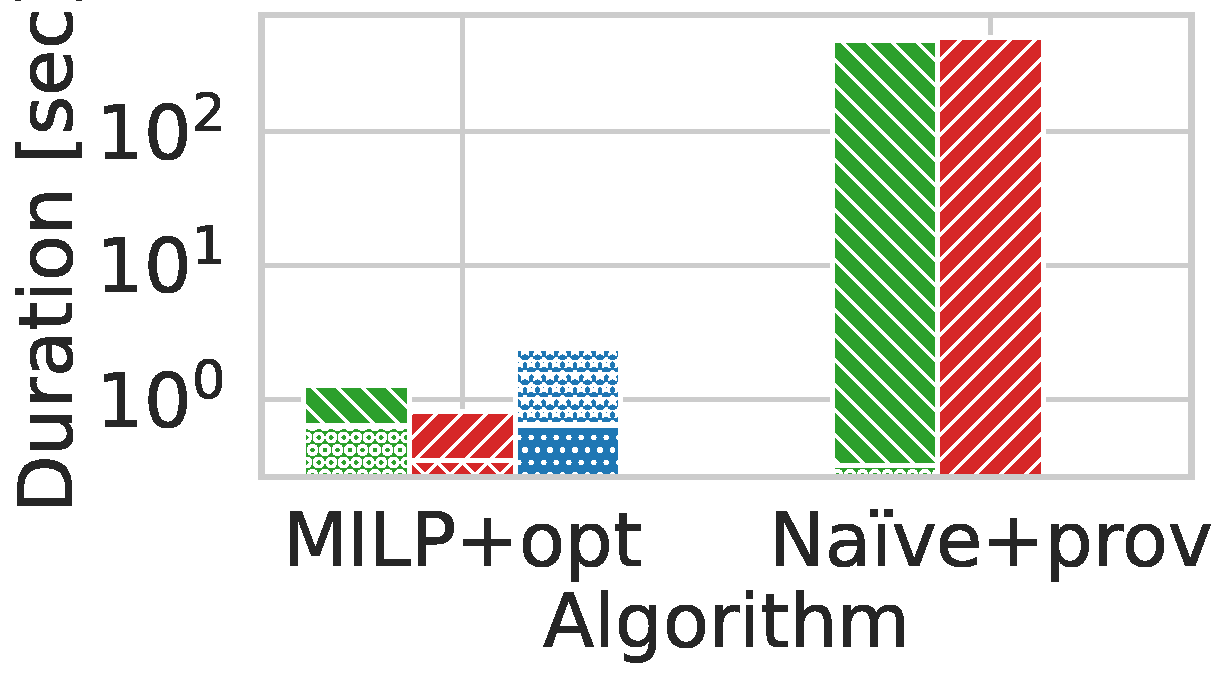
\includegraphics[width=.75\linewidth]{figures/law_method.pdf}
      \caption{Law Students}
      \label{fig:law_method}
    \end{subfigure}
    \begin{subfigure}{.35\textwidth}
      \centering
      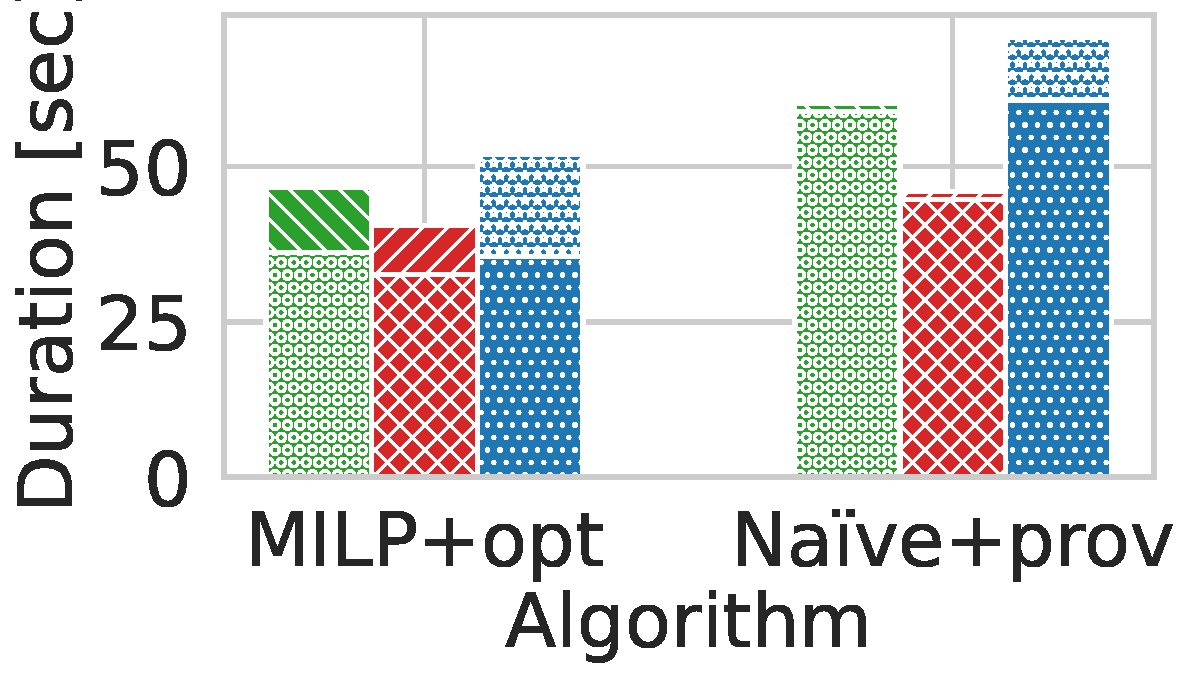
\includegraphics[width=.75\linewidth]{figures/meps_method.pdf}
      \caption{MEPS}
      \label{fig:meps_method}
    \end{subfigure}%
    \begin{subfigure}{.35\textwidth}
      \centering
      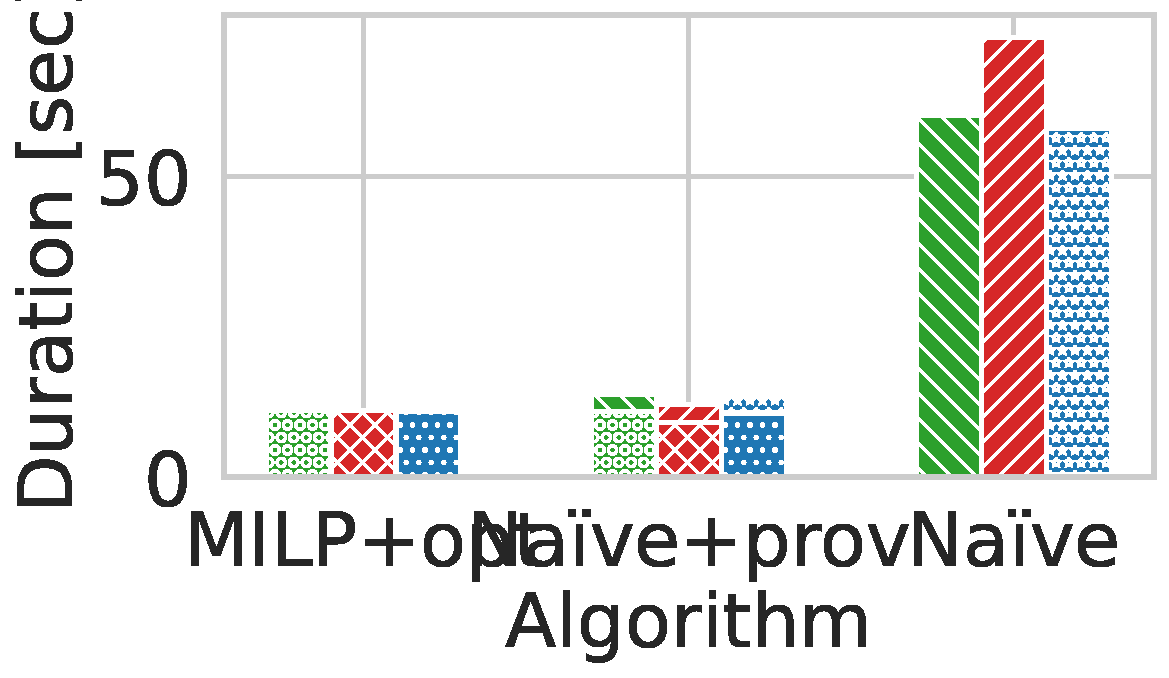
\includegraphics[width=.75\linewidth]{figures/tpch_method.pdf}
      \caption{TPC-H}
      \label{fig:r4}
    \end{subfigure}
    \caption{Running time of compared algorithms, for cases where computation completed within a 1-hour timeout (method or distance omitted when timed out).  MILP+opt consistently outperforms other methods.}
    \label{fig:time_vs_method}
\end{figure}
\paragraph*{\textbf{Running time for compared algorithms}}
We begin by comparing the running time of all algorithms using the default parameters and setting a timeout of one hour. 
Recall that the size of the generated MILP program (without optimization) is linear in the data size and that MILP solvers are typically sensitive to the program size. Thus, we expect the MILP algorithm to struggle with large-scale datasets. On the other hand, the na\"{i}ve approaches perform a brute-force search over the possible refinements, where their number is exponential in the number of predicates in the query (and their domain). Thus, datasets with high cardinality in the domain of the query predicate are likely to be challenging for the na\"{i}ve solutions.  

Figure~\ref{fig:r1} presents performance for the Astronauts dataset. The optimized MILP solution outperforms the unoptimized MILP, and we observe a speedup of up to 6 times. Given that there are $114$ different values for ``Graduate Major'', the space of refinements is extremely large and both Na\"{i}ve and Na\"{i}ve+prov timed out (and thus omitted from the graph). \Cref{fig:law_method,fig:meps_method,fig:r4} show the results for the remaining datasets. In these cases, due to the data size, the unoptimized MILP was unable to terminate before the time-out. MEPS and TPC-H have a relatively small space of refinements for the posed queries, making Na\"{i}ve+prov competitive with MILP+opt. However, Law Students has a considerably larger space of refinements (although modest compared to Astronauts), making Na\"{i}ve time out and Na\"{i}ve+prov significantly slower than MILP+opt. Essentially, MILP+opt is well-posed to deal with scaling both the data size and the space of the possible refinements.
The na\"{i}ve brute-force search methods and unoptimized MILP method fail to scale, and we exclude them from the rest of the experiments.


\begin{figure*}[t]
    \begin{subfigure}{.35\textwidth}
      \centering
      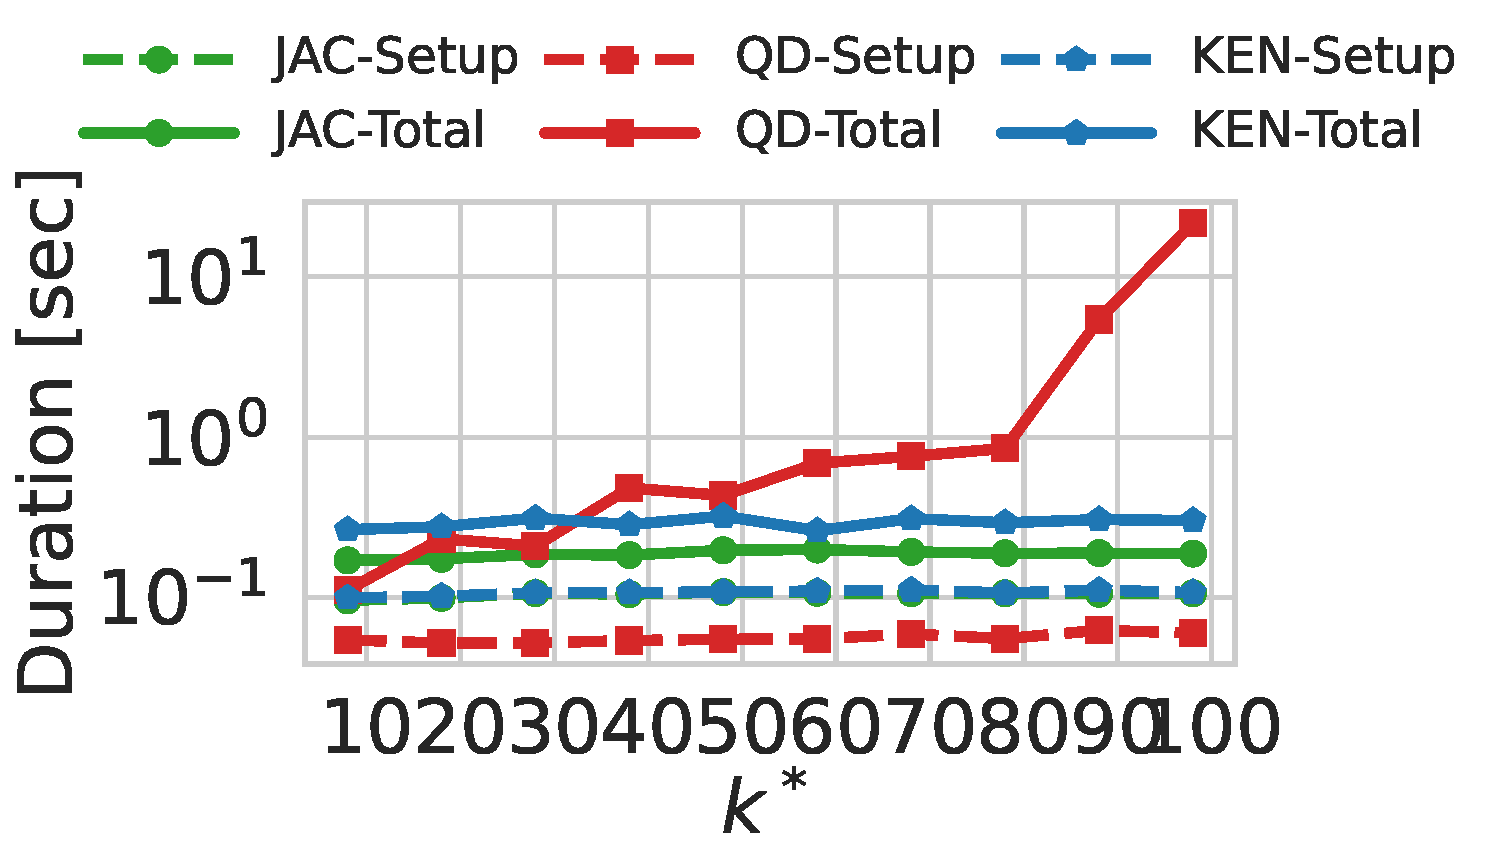
\includegraphics[width=.87\linewidth]{figures/astr_k.pdf}
      \hspace{-0.54cm}
      \caption{Astronauts (log scale)}
      \label{fig:r5}
    \end{subfigure}
    \begin{subfigure}{.35\textwidth}
      \centering
      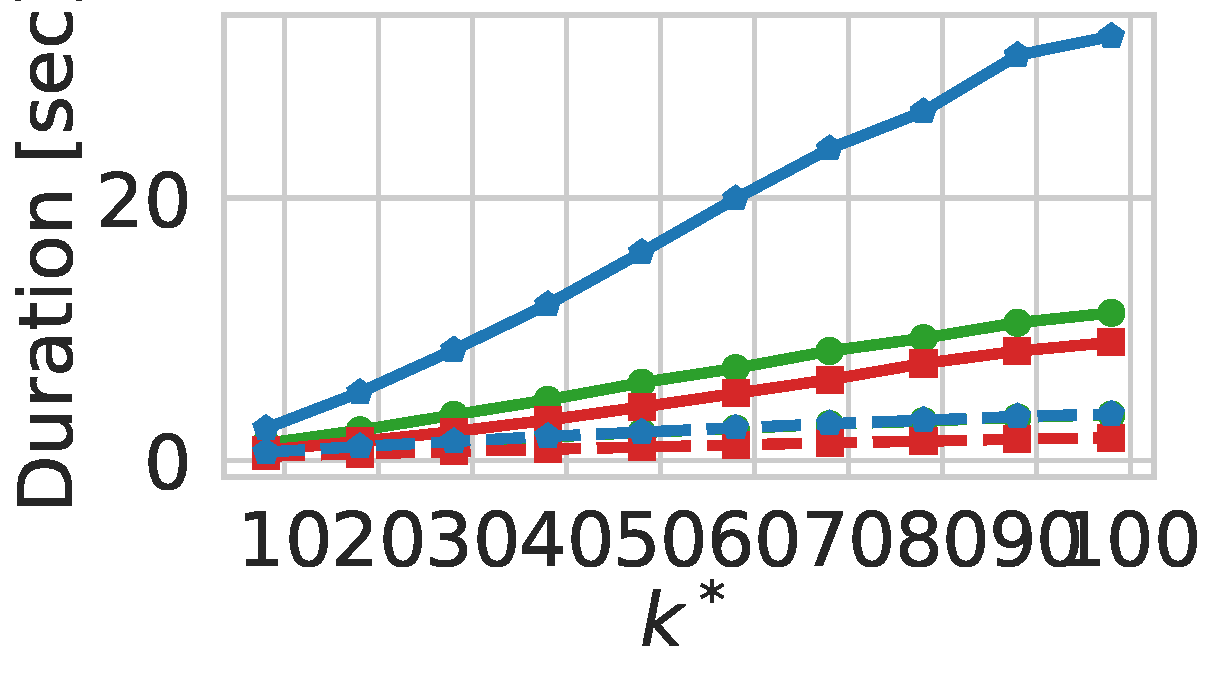
\includegraphics[width=.75\linewidth]{figures/law_k.pdf}
      \caption{Law Students}
      \label{fig:r6}
    \end{subfigure}
    \begin{subfigure}{.35\textwidth}
      \centering
      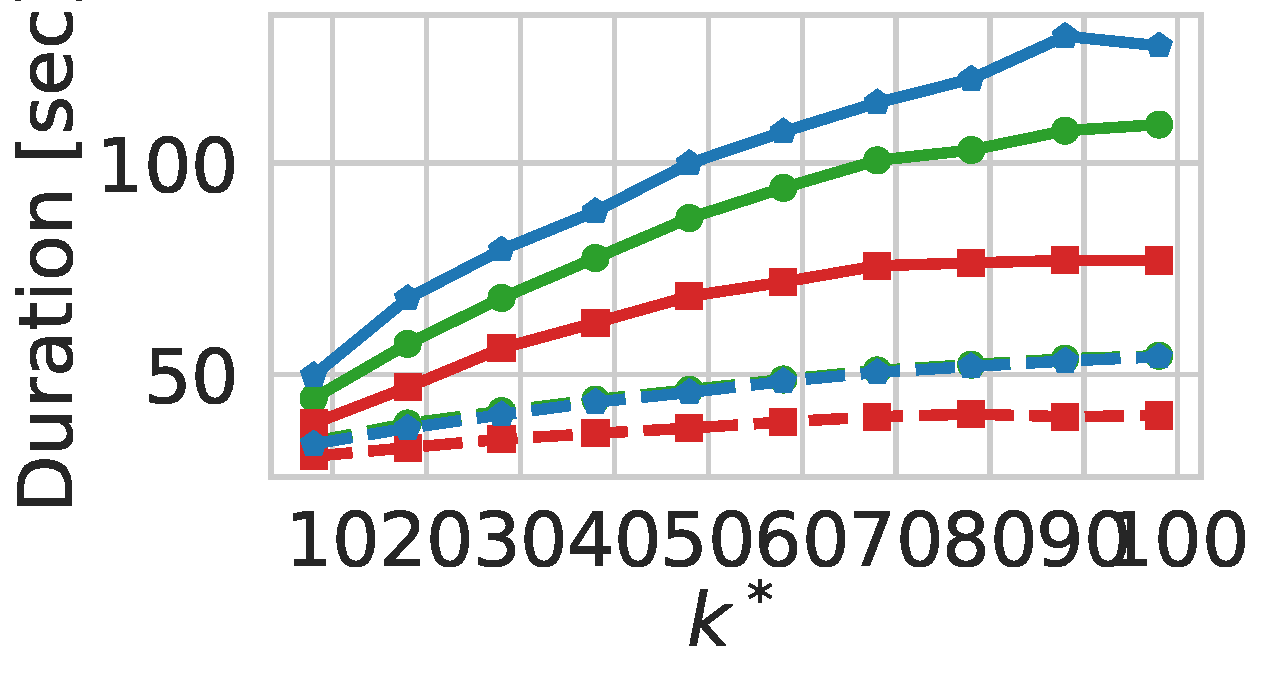
\includegraphics[width=.75\linewidth]{figures/meps_k.pdf}
      \caption{MEPS}
      \label{fig:r7}
    \end{subfigure}
    \begin{subfigure}{.35\textwidth}
      \centering
      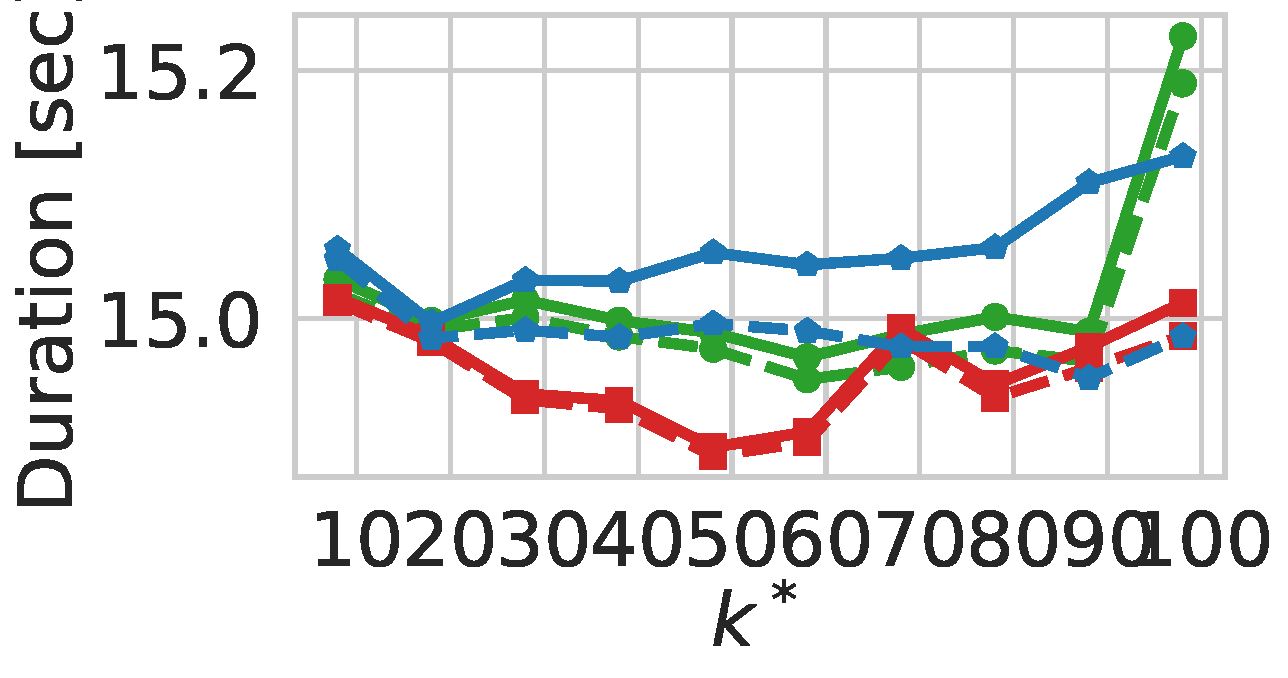
\includegraphics[width=.75\linewidth]{figures/tpch_k.pdf}
      \caption{TPC-H}
      \label{fig:r8}
    \end{subfigure}

    \caption{Running time vs. $k^*$, showing $DIS_{pred}$ is often the fastest to compute, while $DIS_{Kendall}$ can be sensitive to increasing $k^*$.}
    \label{fig:time_vs_k}
\end{figure*}
\paragraph*{\textbf{Effect of $k^*$}}
We study the effect of $k^*$, the largest $k$ with a constraint in the constraint set, on the running time of our algorithm by increasing the parameter $k$ of the constraint from $10$ to $100$ in increments of $10$. The results are presented in Figure~\ref{fig:time_vs_k}. Recall that the relevancy-based optimization from \Cref{sec:optimizations} aims at reducing the program size using $k^*$. 
We expect to see its effect degrade as $k^*$ increases, as shown in \Cref{fig:r6,fig:r7}. 
The optimization is less effective for  Astronauts (Figure~\ref{fig:r5}), as the number of different lineage equivalent classes is large, and each consists of a relatively small number of tuples (fewer than $10$). 
Therefore, the expressions generated for very few tuples may be removed from the program. The optimization is particularly effective for $Q_5$ of TPC-H (\Cref{fig:r8}), as the vast majority of expressions are removed as there are only $5$ lineage equivalence classes. Moreover, we see that most of the time is spent setting up the problem rather than solving it.


\begin{figure*}[t]
    \begin{subfigure}{.35\textwidth}
      \centering
      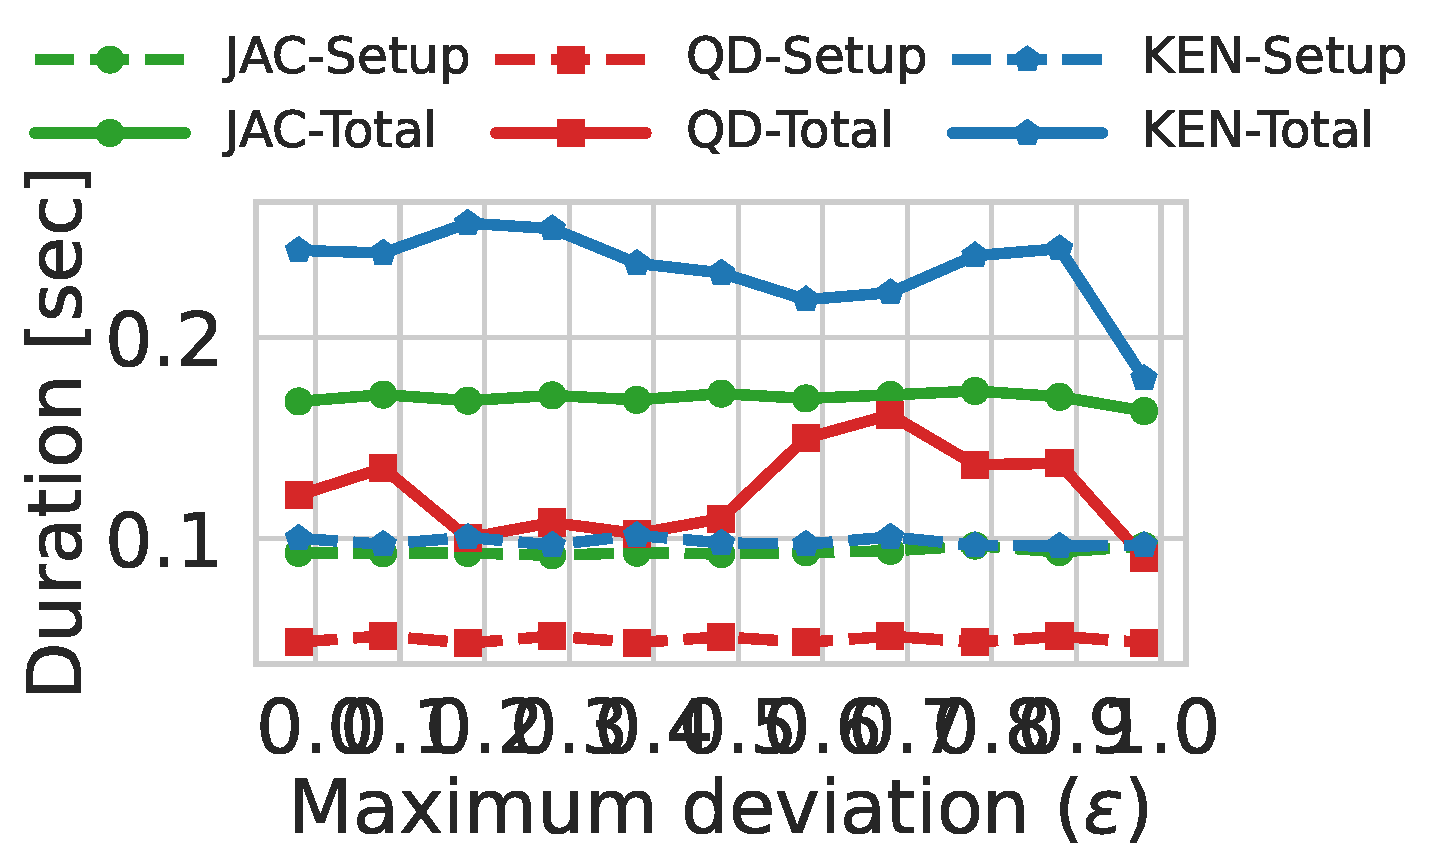
\includegraphics[width=.87\linewidth]{figures/astr_eps.pdf}
      \hspace{-0.54cm}
      \caption{Astronauts}
      \label{fig:r9}
    \end{subfigure}
    \begin{subfigure}{.35\textwidth}
      \centering
      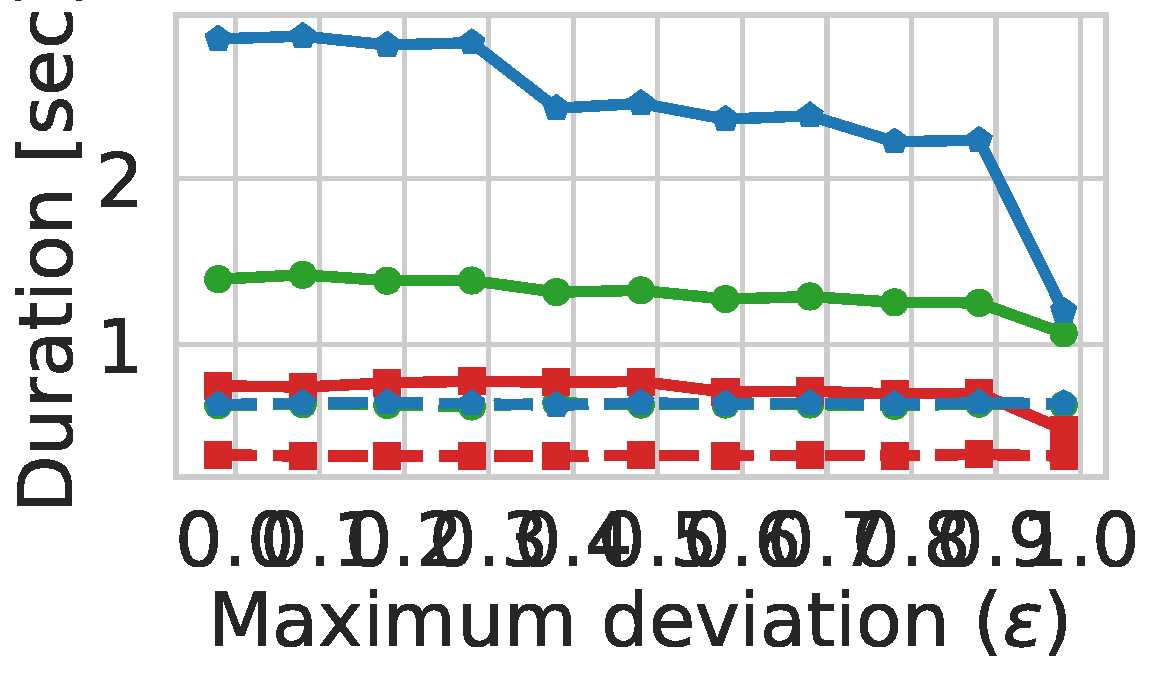
\includegraphics[width=.75\linewidth]{figures/law_eps.pdf}
      \caption{Law Students}
      \label{fig:r10}
    \end{subfigure}
    \begin{subfigure}{.35\textwidth}
      \centering
      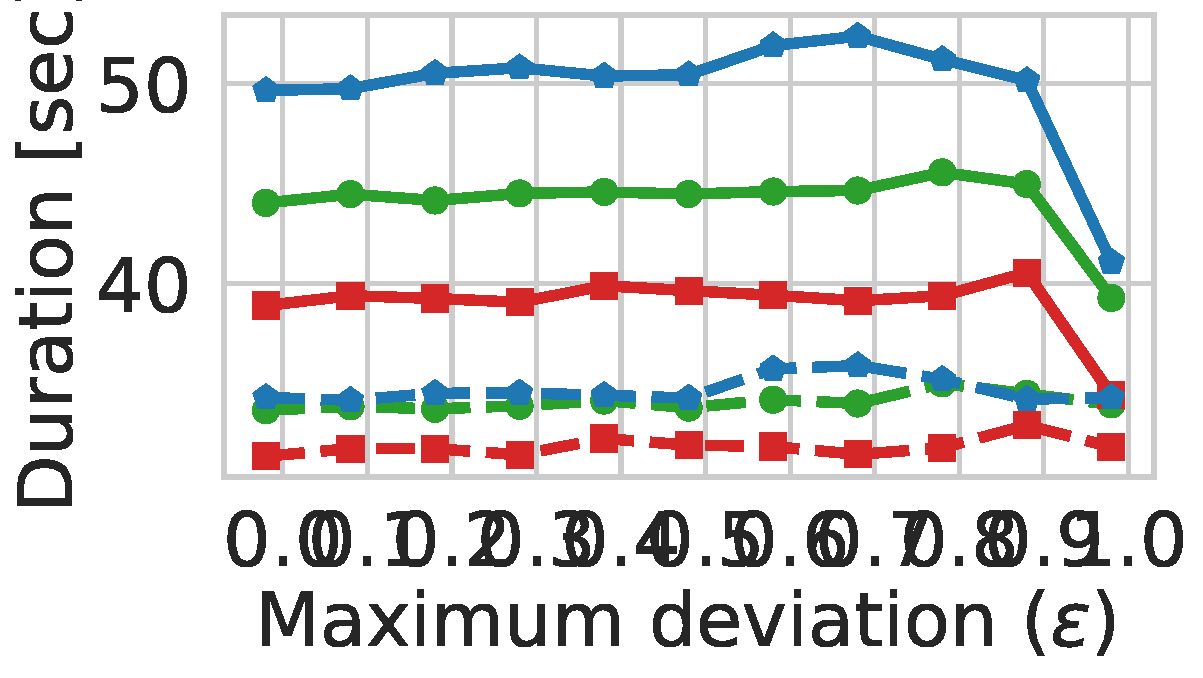
\includegraphics[width=.75\linewidth]{figures/meps_eps.pdf}
      \caption{MEPS}
      \label{fig:r11}
    \end{subfigure}
    \begin{subfigure}{.35\textwidth}
      \centering
      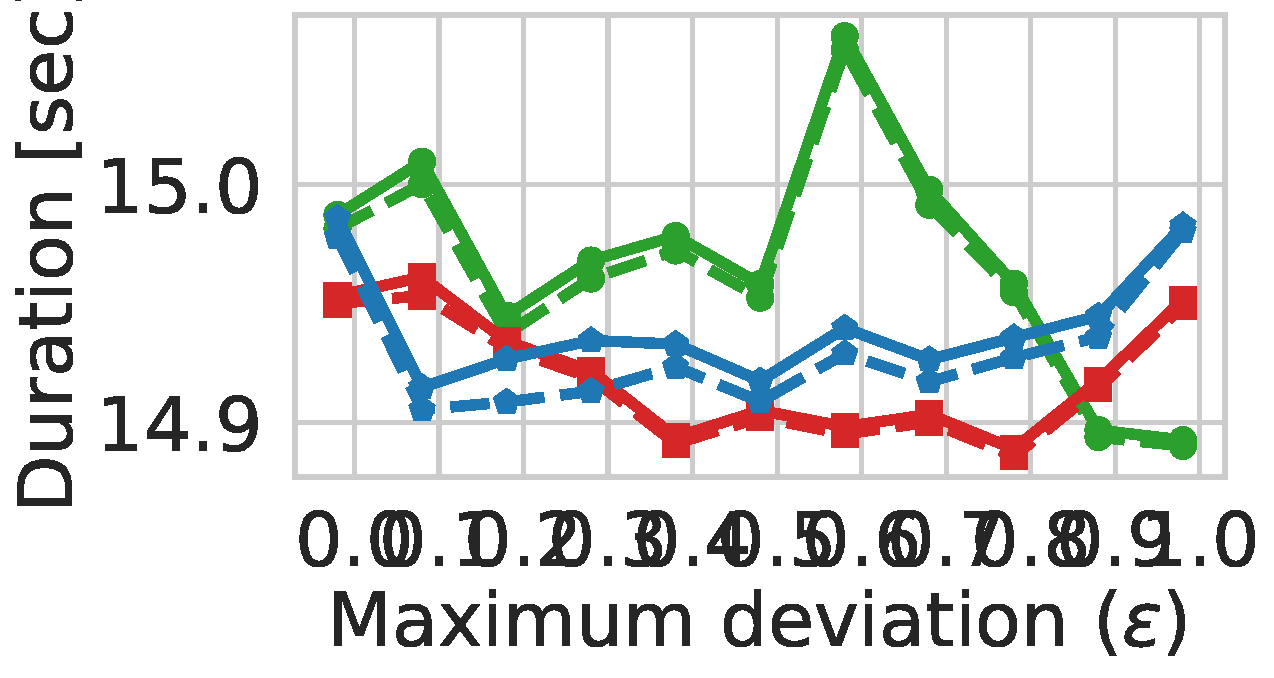
\includegraphics[width=.75\linewidth]{figures/tpch_eps.pdf}
      \caption{TPC-H}
      \label{fig:r12}
    \end{subfigure}
    
    \caption{Running time vs. maximum deviation ($\varepsilon$), showing that the effect of $\varepsilon$ is limited.}
    \label{fig:time_vs_eps}
\end{figure*}
\paragraph*{\textbf{Effect of maximum deviation ($\varepsilon$)}}
\label{sec:time_vs_eps}
While an increase in $\varepsilon$ may make finding feasible refinements easier, the solver must still find the minimal refinement, which remains a difficult task. Therefore, the value of $\varepsilon$ should not significantly affect the running time. Figure~\ref{fig:time_vs_eps} shows that the running time is fairly stable. We observed a decrease when $\varepsilon$ reaches $1.0$. This is because we use only lower-bound constraints in this experiment, where the deviation of any (refined) query is bounded by $1.0$, i.e. finding a satisfying refinement is trivial as all refinements are good enough.
In \Cref{fig:r12}, 
the solver time is negligible and depends mostly on the setup time, which is very similar across all values of $\varepsilon$ (differing by at most $1\%$).



\begin{figure*}[t]
    \begin{subfigure}{.35\textwidth}
      \centering
      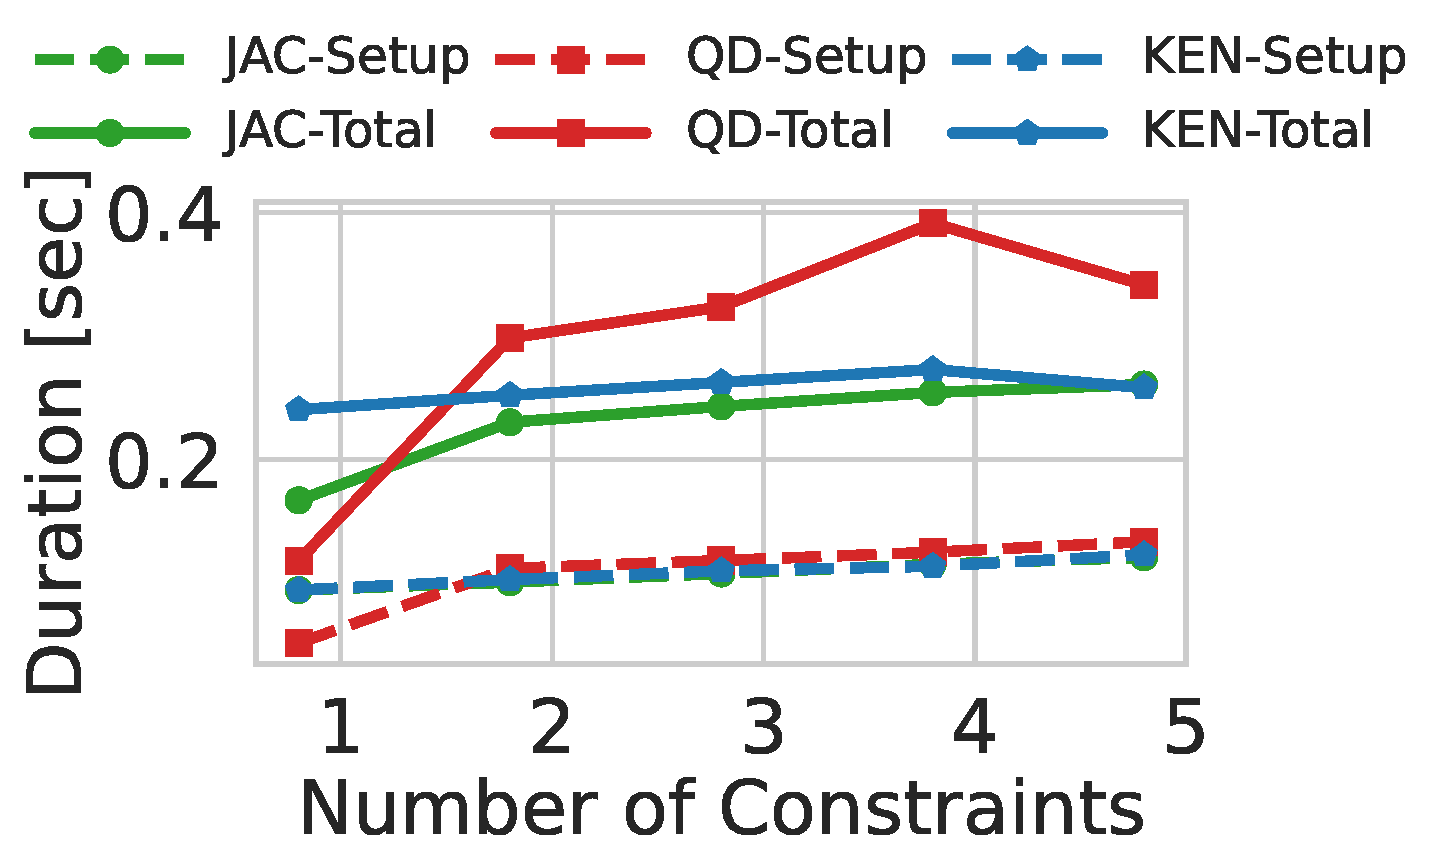
\includegraphics[width=.87\linewidth]{figures/astr_num.pdf}
      \hspace{-0.54cm}
      \caption{Astronauts}
      \label{fig:r13}
    \end{subfigure}
    \begin{subfigure}{.35\textwidth}
      \centering
      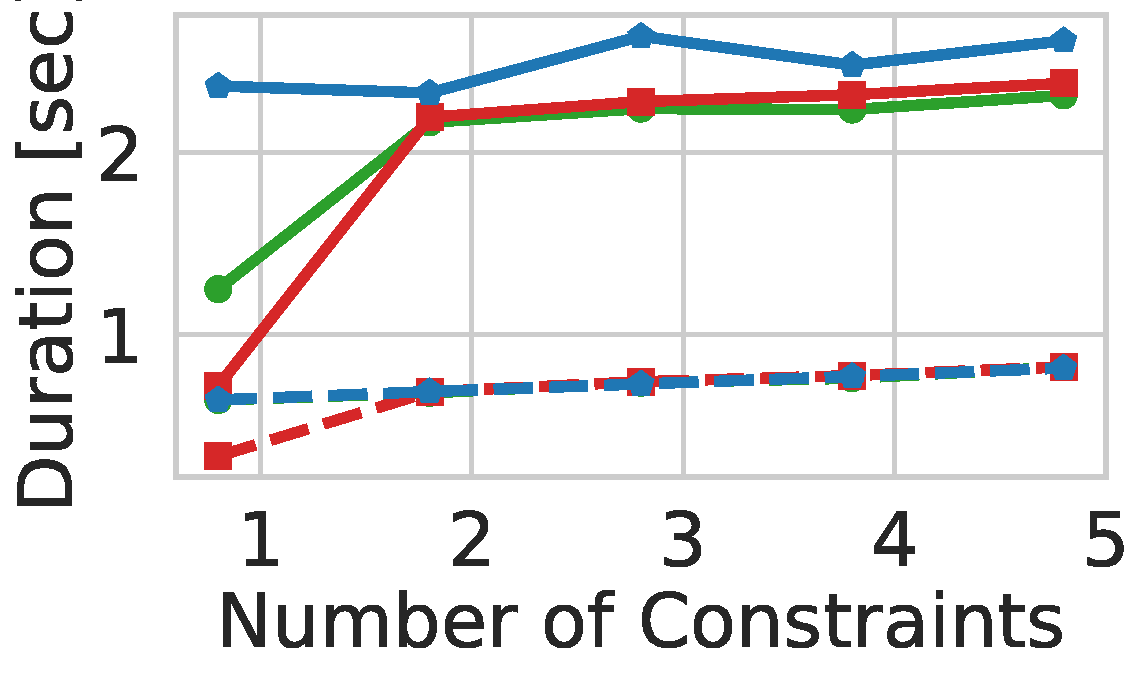
\includegraphics[width=.75\linewidth]{figures/law_num.pdf}
      \caption{Law Students}
      \label{fig:r14}
    \end{subfigure}
    \begin{subfigure}{.35\textwidth}
      \centering
      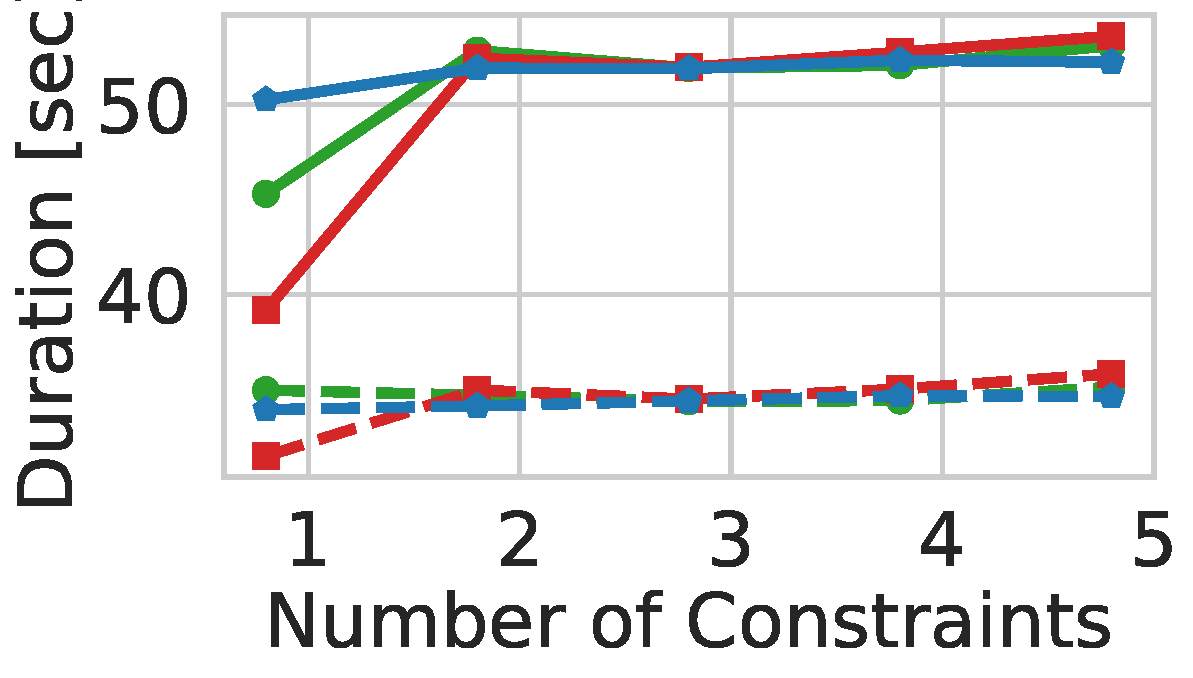
\includegraphics[width=.75\linewidth]{figures/meps_num.pdf}
      \caption{MEPS}
      \label{fig:r15}
    \end{subfigure}
    \begin{subfigure}{.35\textwidth}
      \centering
      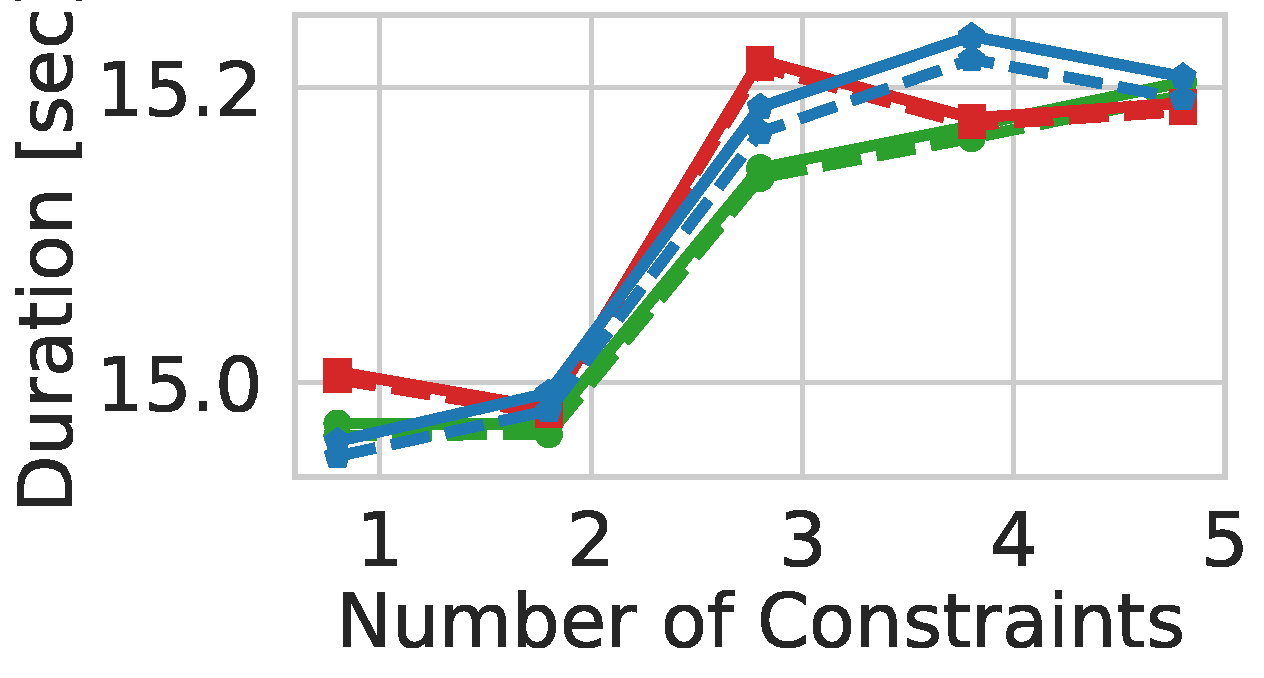
\includegraphics[width=.75\linewidth]{figures/tpch_num.pdf}
      \caption{TPC-H}
      \label{fig:r16}
    \end{subfigure}
    
    \caption{Running time vs. the number of constraints: the impact of the number of constraints is limited.}
    \label{fig:time_vs_num_of_constraints}
\end{figure*}
\paragraph*{\textbf{Effect of constraint quantity}}
The number of generated expressions of the form (\ref{eq:in_prefix_inline}) and (\ref{eq:tuples_to_satisfy_inline}) is linear in the number of constraints. Thus, when increasing the number of constraints, the program size increases and as a result, we expect to see an increase in the running time.
We gradually added constraints to the constraint set in the order they listed in Table~\ref{tab:queriesAndConstraints}. To ensure that the set of constraints can be satisfied along with the default value of $\varepsilon$, we slightly adjust the value of the first two constraints for Astronauts, Law Students, and MEPS to have a lower-bound of $\frac{k}{3}$. As shown in Figure~\ref{fig:time_vs_num_of_constraints}, we observed a slight increase in the running time as the number of constraints increased in contrast to increasing the value of $k$. The number of expressions is linear in the number of constraints and tuples, however there are significantly fewer constraints than tuples, which is why the number of constraints does not have a pronounced effect on the runtime.
TPC-H (\Cref{fig:r16}) shows a negligible difference as the vast majority of the time is set up the MILP problem, as the solver has only $5$ lineage equivalence classes to explore.

\begin{figure*}[t]
    \begin{subfigure}{.35\textwidth}
      \centering
      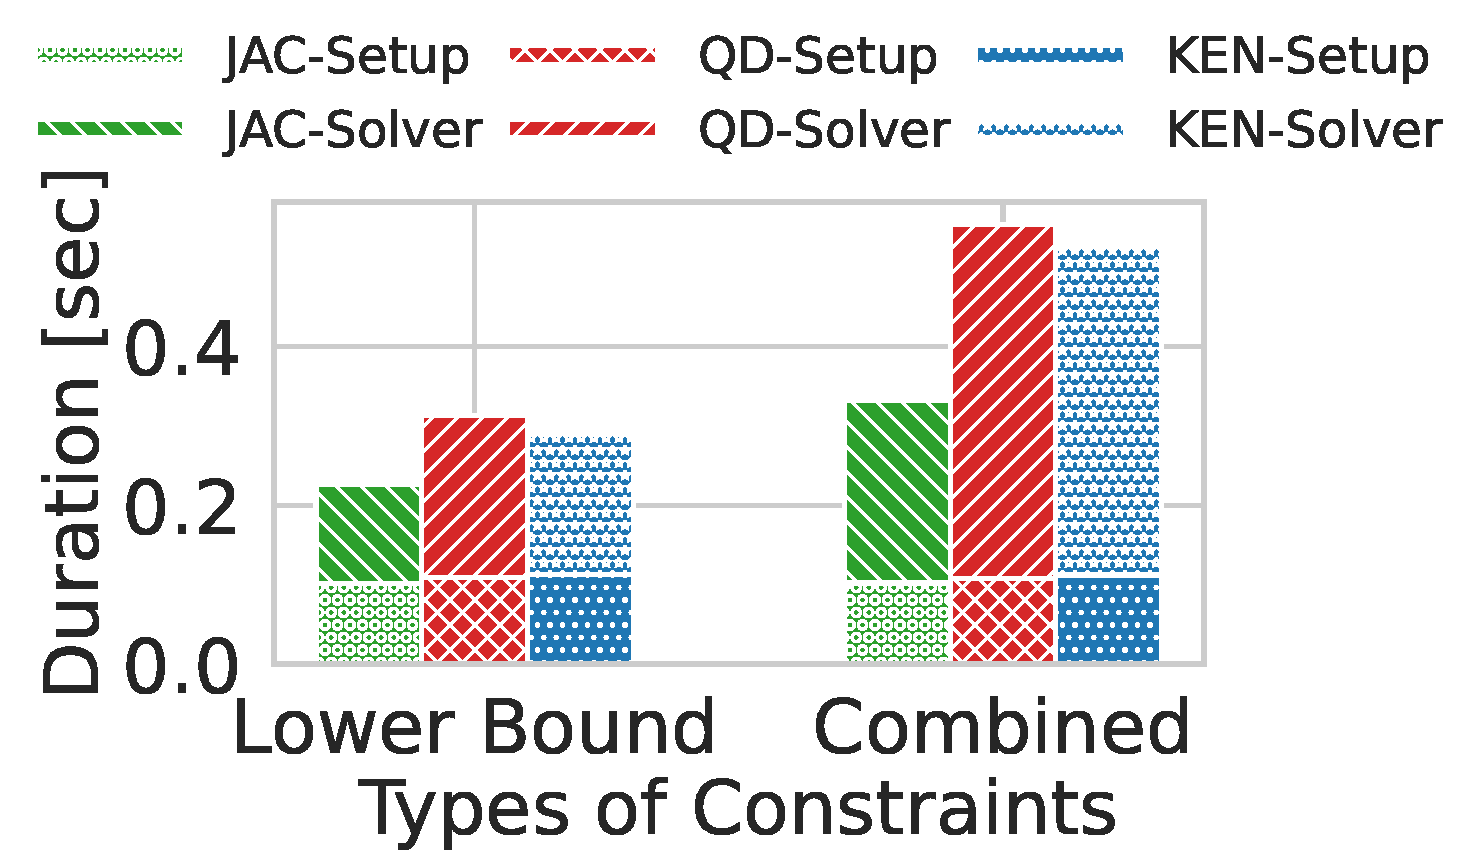
\includegraphics[width=.87\linewidth]{figures/astr_const_type.pdf}
      \hspace{-0.65cm}
      \caption{Astronauts}
      \label{fig:r17}
    \end{subfigure}
    \begin{subfigure}{.35\textwidth}
      \centering
      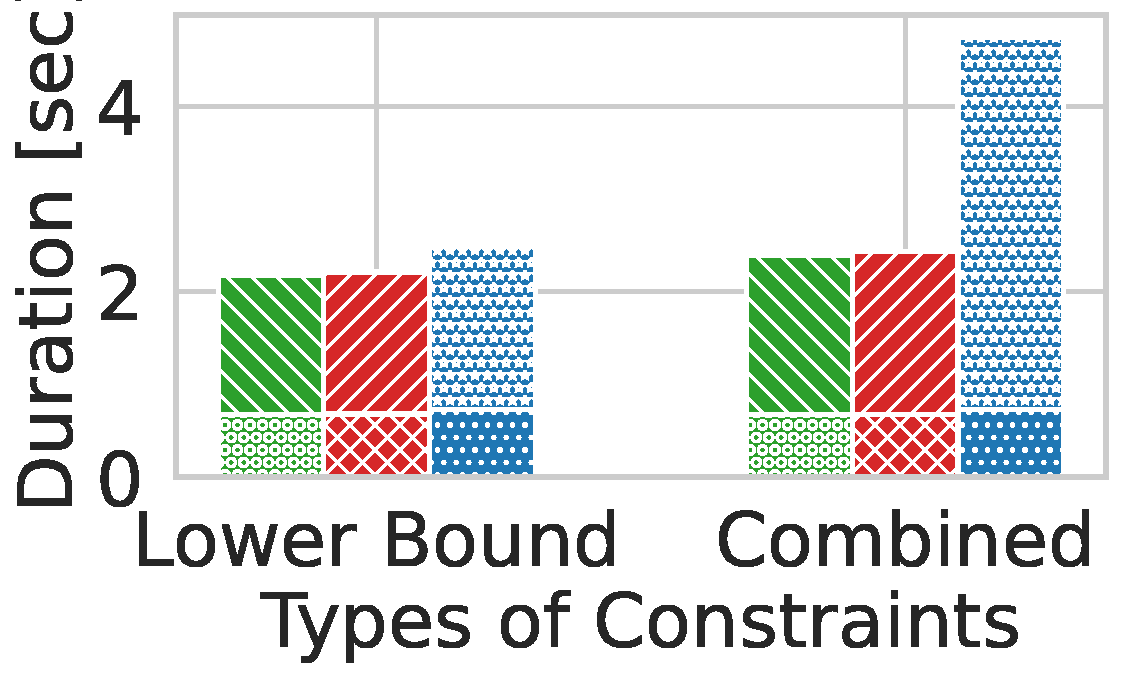
\includegraphics[width=.75\linewidth]{figures/law_const_type.pdf}
      \caption{Law Students}
      \label{fig:r18}
    \end{subfigure}
    \begin{subfigure}{.35\textwidth}
      \centering
      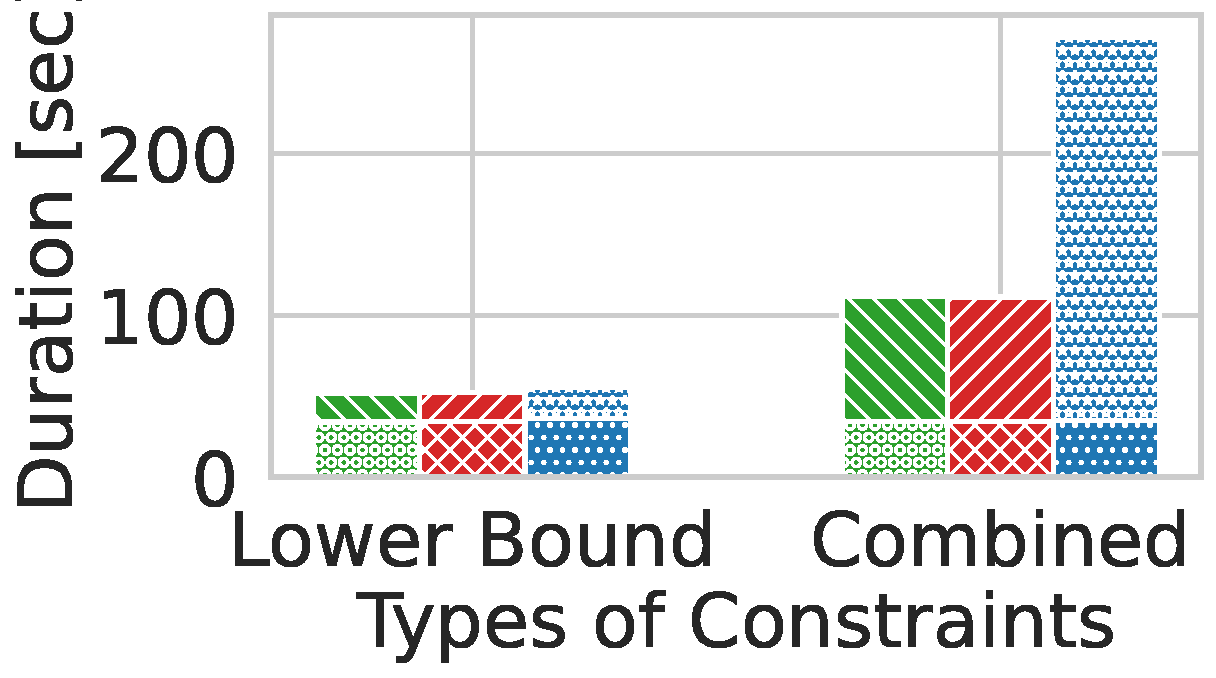
\includegraphics[width=.75\linewidth]{figures/meps_const_type.pdf}
      \caption{MEPS}
      \label{fig:r19}
    \end{subfigure}
    \begin{subfigure}{.35\textwidth}
      \centering
      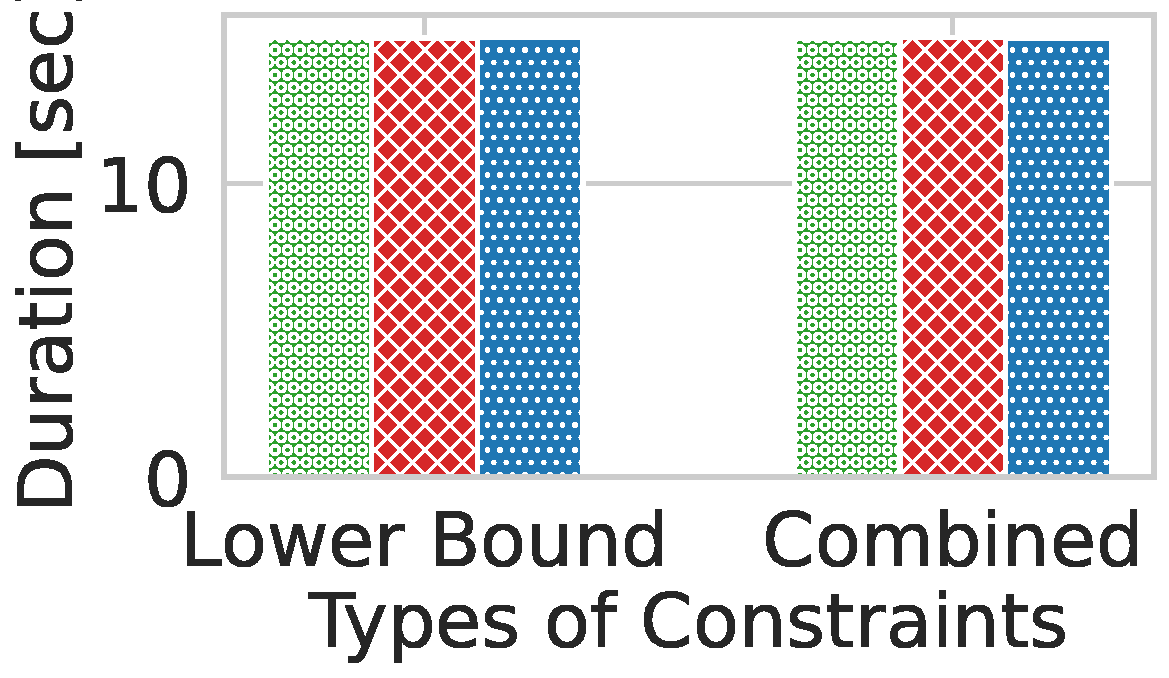
\includegraphics[width=.75\linewidth]{figures/tpch_const_type.pdf}
      \caption{TPC-H}
      \label{fig:r20}
    \end{subfigure}
    
    \caption{Running time vs. constraint type, showing the efficacy of one of our optimizations.}
    \label{fig:time_vs_constraint_type}
\end{figure*}
\paragraph*{\textbf{Effect of constraint types}}
In \Cref{sec:optimizations}, we presented an optimization that is effective when tuples belong to groups with only either lower-bound or upper-bound constraints made on them. To demonstrate the effect of this optimization, we generate two sets of constraints for each dataset: $\constraints_{L}$ with lower bound constraints only, and $\constraints_{M}$ with a mixed set of upper bound and lower bound constraints. In particular, each dataset, $\constraints_{L}$ includes constraints (1) and (2) from Table~\ref{tab:queriesAndConstraints}, and $\constraints_{M}$ includes constraints (1) and (2), where constraint (2) is turned into an upper-bound constraint. 
Notice that these particular attributes are binary, and, as we assume there are at least $k^*$ tuples in the output, the two constraints of $\constraints_{M}$ are equivalent (except for TPC-H, which lacks any binary attributes). We then compared the running time when using $\constraints_{L}$ and $\constraints_{M}$ (for which the optimization was disabled for $\constraints_{M}$). The results are presented in \Cref{fig:time_vs_constraint_type}. As expected, the running times for the case of $\constraints_{L}$ are typically better, as shown in \Cref{fig:r17,fig:r18,fig:r19}, indicating the usefulness of the optimization. We note that the experiment in \Cref{fig:r20} depicting the experiment for TPC-H shares the same performance characteristics as the previous experiments.



\begin{figure*}[t]
    \begin{subfigure}{.35\textwidth}
      \centering
      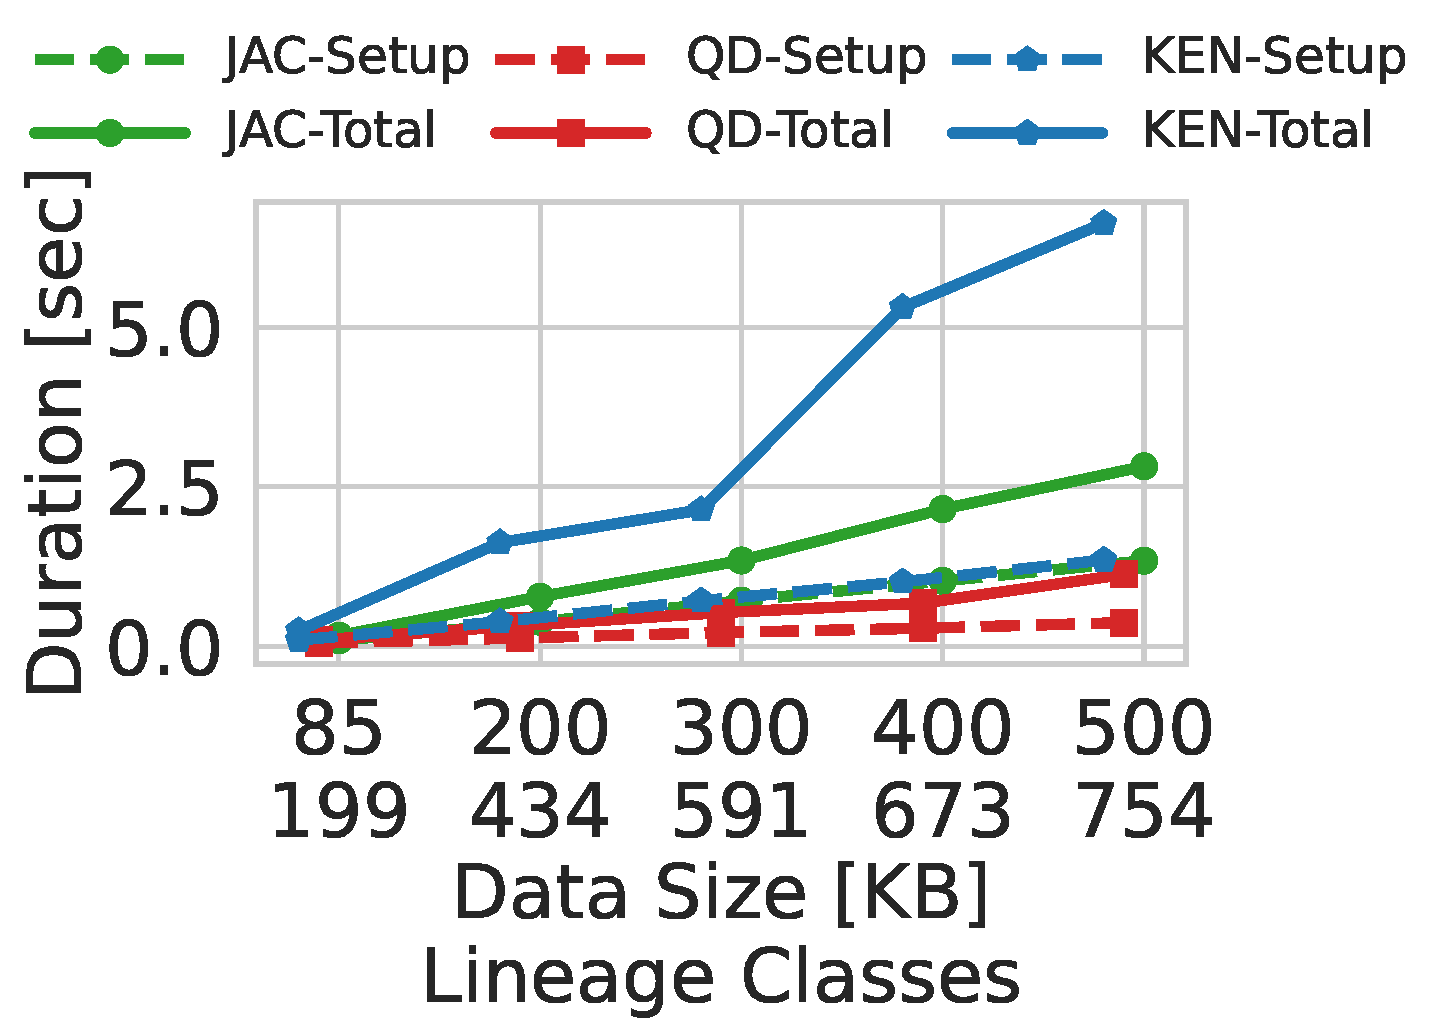
\includegraphics[width=.87\linewidth]{figures/astr_size.pdf}
      \hspace{-0.51cm}
      \caption{Astronauts}
      \label{fig:r21}
    \end{subfigure}
    \begin{subfigure}{.35\textwidth}
      \centering
      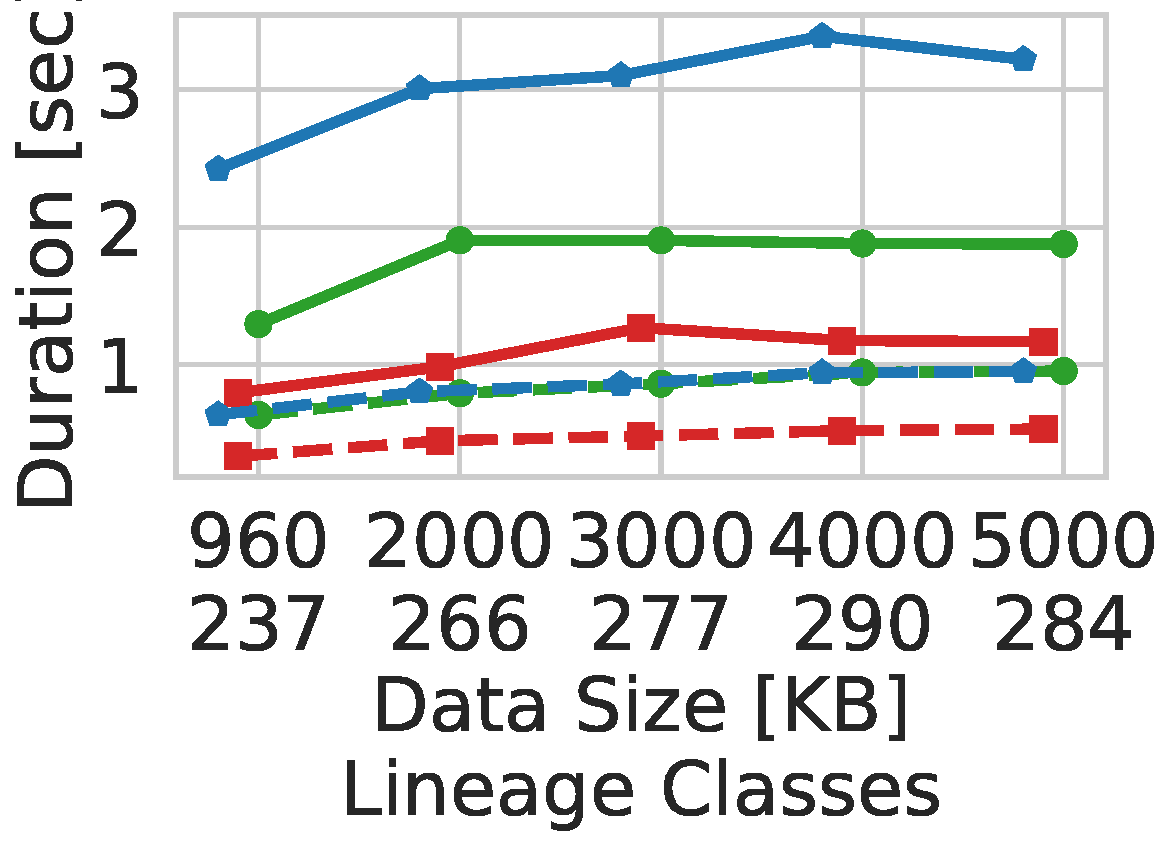
\includegraphics[width=.75\linewidth]{figures/law_size.pdf}
      \caption{Law Students}
      \label{fig:r22}
    \end{subfigure}
    \begin{subfigure}{.35\textwidth}
      \centering
      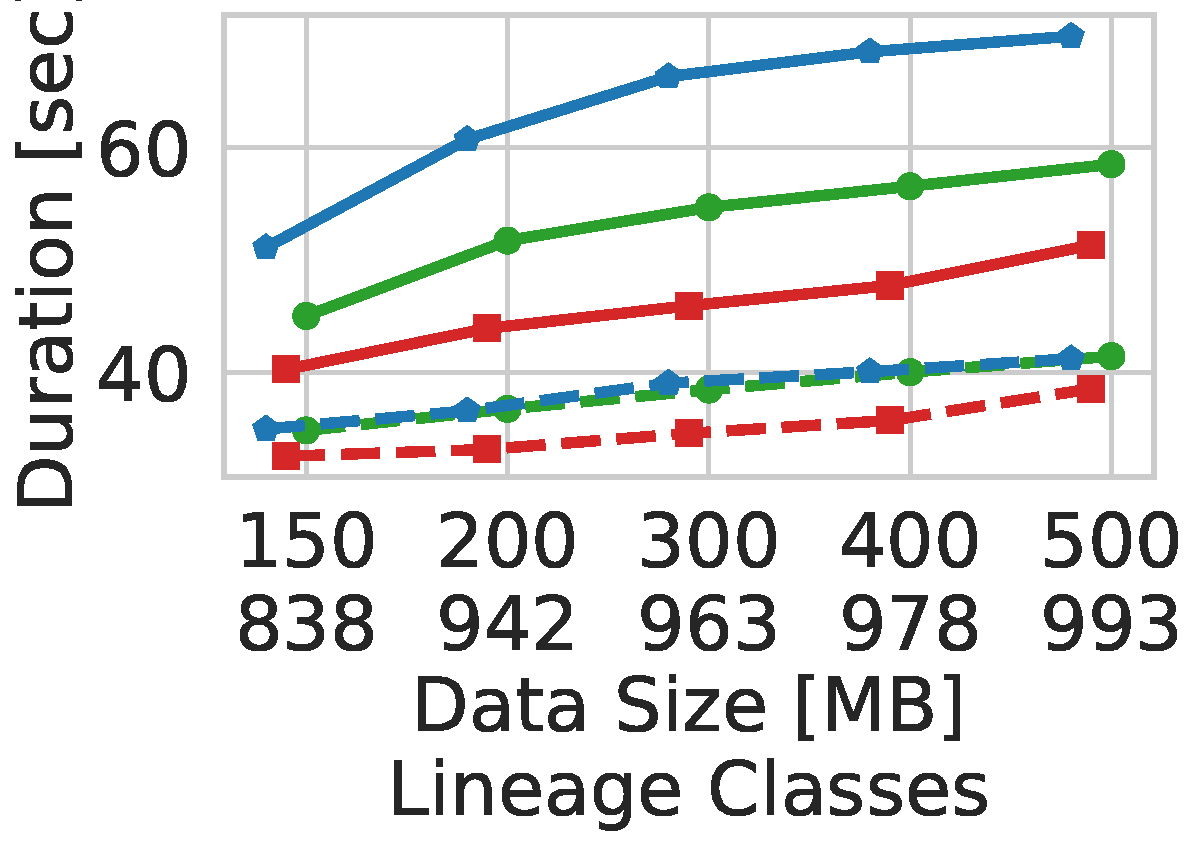
\includegraphics[width=.75\linewidth]{figures/meps_size.pdf}
      \caption{MEPS}
      \label{fig:r23}
    \end{subfigure}
    \begin{subfigure}{.35\textwidth}
      \centering
      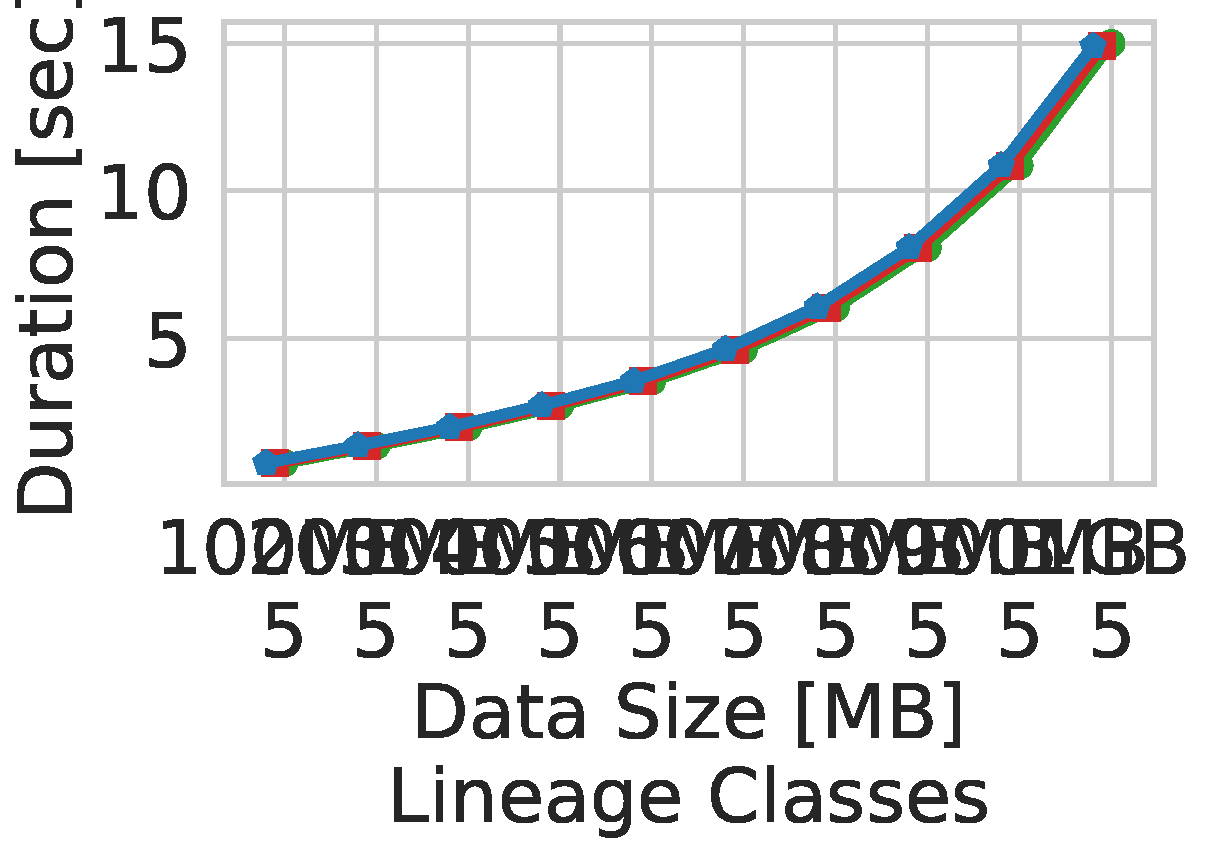
\includegraphics[width=.75\linewidth]{figures/tpch_size.pdf}
      \caption{TPC-H}
      \label{fig:r24}
    \end{subfigure}
    
    \caption{Running time vs. data size. The setup time is mostly impacted by the cost to capture lineage from the input query, while the solving time is mostly impacted by the number of lineage classes.}
    \label{fig:time_vs_size}
\end{figure*}
\paragraph*{\textbf{Effect of dataset size}}
We use SDV~\cite{SDV} to synthesize scaled-up versions of the real datasets. Not only does this increase the data size, but new lineage classes are created according to the distribution of the dataset as well. For TPC-H, we generate different scales of the dataset according to its standard, but no new lineage classes are created. The number of variables and expressions of the generated MILP is linear in the number of tuples in the dataset. However, given that solving MILP is in ${\sf NP}$, we expect a non-polynomial increase in running time with an increase in the data size. 
The results are plotted in \Cref{fig:time_vs_size}, each plot starting from the original size of the dataset. For the Astronauts, Law Students, and MEPS datasets, we observed a modest increase in the runtime as the data size grows. This could be explained by the low increase in the number of lineage classes, which impacts the efficiency of our optimization and has a greater effect on the running time.
In TPC-H (Figure~\ref{fig:r24}), the vast majority of the running time is spent building the MILP problem, and in this case, constructing the set of lineages for Q5 involves a non-trivial amount of join processing.

\paragraph*{\textbf{Effect of chosen distance measure}}
We observed that in most cases, $DIS_{Kendall}$ is the hardest to compute as it involves extra variables in order to linearize the measure. When the refinement space is extremely large, such as for Astronauts,  $DIS_{pred}$ takes longer to prove optimality (as seen in \Cref{fig:r5,fig:r13}).

\subsection{Comparison with Erica \cite{ERICA,ERICAfull}}
\label{sec:erica_comparison}
We conclude with a comparison to 
Erica~\cite{ERICA,ERICAfull}, which presents a similar framework for query refinements to satisfy cardinality constraints over groups representation in the query's output. We note Erica focuses on cardinality constraints over the {\it entire} output, without considering the order of tuples. By restricting the overall output size to $k$, Erica may be used to refine a given query to satisfy constraints over the top-$k$ tuples. However, as we next demonstrate, this additional constraint over the output size also limits the possible refinements to those that have at most $k$ tuples. Moreover, this adjustment of Erica cannot be used to constrain over different values of $k$ simultaneously (as in our running example). Additionally, since satisfying the constraints in our setting is more challenging, we focus on finding approximate solutions that are close to satisfying the constraints, while Erica only finds solutions that satisfy the constraints exactly. Finally, our framework allows the user to define different distance measures between queries whereas Erica uses a single distance measure based on the predicate distance.
We compare the systems by refining the query $Q_L$ except with the predicates {\tt Region = `GL' AND GPA >= 3.0}.
subject to the singleton constraint set $\constraints = \{ \lb{Sex='F'}{k=100} = 50 \}$. To be consistent with~\cite{ERICA,ERICAfull}, we aim to minimize the predicate distance (using $DIS_{pred}$ as the distance measure) and allow only results that satisfy the constraints exactly, i.e., $\varepsilon = 0$. When running Erica, we added a constraint requiring that exactly $100$ results are returned to ensure the top-$100$ tuples contains at least $50$ female candidates, and that there are enough results to satisfy the assumption in our problem definition. 
Using our optimized MILP-based approach, we were able to find a minimal refinement in $\approx 11$ seconds. The refinement selects candidates from the regions {\tt `GL'} or {\tt `SC'} with a GPA of at least $4.0$. Erica found $5$ different refinements in $\approx 53$ seconds, though none of them are closer to $Q$ than the refinement found by our framework. In fact, all of the refinements require a GPA of at least $4.0$ and select {\it 3} regions. The refinement found by our system was not generated by Erica due to the additional constraint requiring the output size to be exactly $100$.



